\documentclass[11pt]{article}
\usepackage[T1]{fontenc}
\usepackage{lmodern}
\usepackage[letterpaper,margin=0.85in]{geometry}
\usepackage{amsmath,amssymb,booktabs,tabularx,graphicx,pdflscape}
\usepackage[hidelinks]{hyperref}
\setlength{\emergencystretch}{2em}
\hypersetup{
  pdftitle={Spectrally constrained stochastic factorization for low-dose CT}
}

\newcommand{\ctfigure}[3]{%
  \begin{figure}[!htp]
    \centering
    \includegraphics[page=#1,width=\linewidth,height=0.77\textheight,keepaspectratio]{ct_sframes_figures.pdf}
    \caption{#3}\label{#2}
  \end{figure}
  \clearpage
}

\begin{document}
\begin{center}
  \Large\bfseries Spectrally constrained stochastic factorization for low-dose CT
\end{center}

\section{Low-dose CT reconstruction model}
\label{sec:ct-model}

We reconstruct the X-ray attenuation of a two-dimensional slice from low-dose measurements taken at multiple angles. The unknown image \(X\) represents attenuation on a \(512\times512\) grid.

\paragraph{What the scanner measures.}
An attenuation image describes how strongly the material at each location reduces the transmitted X-ray beam per unit distance. At one angular position, called a \emph{view}, an X-ray source illuminates a line of detector bins on the opposite side of the object. The rays from the source to those bins spread out in a fan. Each bin records the intensity transmitted along its ray. In the idealized Beer--Lambert model, dividing the transmitted intensity by the unobstructed intensity and taking the negative logarithm gives the line integral of attenuation along that ray. This is why the processed measurements can be fitted with a linear forward operator in the image \(X\) \cite{detect}.

\paragraph{The forward operator \(P_i\).}
Treat \(X_{pq}\) as the constant attenuation within pixel \((p,q)\). Let \(\ell_{ij,pq}\) be the length in millimeters of ray \(j\) in view \(i\) inside that pixel. The CPU line projector used here applies the map
\begin{equation}
  P_i\colon\mathbb R^{512\times512}\longrightarrow\mathbb R^{d},
  \qquad
  [P_i(X)]_j=\sum_{p,q}\ell_{ij,pq}X_{pq},
  \qquad d=956 .
  \label{eq:ct-ray}
\end{equation}
The weights are fixed by the calibrated source and detector geometry. A ray contributes only to pixels it crosses. ASTRA traces the rays to apply the operator, so the solver can evaluate a selected set of views directly \cite{astra}.

\paragraph{Factorized data fitting.}
We model the image as \(X=UV^\top\), with \(U,V\in\mathbb R^{512\times64}\), to restrict its rank to at most 64. All views of a slice constrain the same two factors. Adding views adds measurements while keeping the factor dimensions fixed.

Let \(\mathcal I_{\rm train}\) be the set of \(N\) training view indices, and let \(y_i\in\mathbb R^d\) be the processed low-dose measurements for view \(i\). Comparing those measurements with the predicted readings gives the unweighted least-squares loss
\begin{equation}
  f(U,V)=\frac{1}{N}\sum_{i\in\mathcal I_{\rm train}} q_i(U,V),
  \qquad
  q_i(U,V)=\frac{\|P_i(UV^\top)-y_i\|_2^2}{2d}.
  \label{eq:ct-loss}
\end{equation}
Each view contributes all its detector bins. The loss is quadratic in the image \(X\). As a function of the factors, it is quartic and nonconvex.

\paragraph{Constraints and the SFRAMES formulation.}
To control the scale of the factors, we cap each factor's operator norm, its largest singular value. We also require the factors to be entrywise nonnegative, which makes the reconstructed attenuation nonnegative. These requirements define
\begin{align}
  C&=\{(U,V):\ \|U\|_{\rm op}\le R_U,\ \|V\|_{\rm op}\le R_V\}, \\
  D&=\{(U,V):\ U\ge 0,\ V\ge 0\}.
\end{align}
We encode nonnegativity by setting \(g=\iota_D\), which is zero on \(D\) and \(+\infty\) elsewhere. This indicator acts directly on the factors, so \(T\) is the identity. With \(x=(U,V)\) and \(f\) given by~\eqref{eq:ct-loss}, the reconstruction problem has the SFRAMES form
\begin{equation}
  \min_{x\in C}\bigl\{f(x)+g(Tx)\bigr\}.
\end{equation}
The component gradients are Lipschitz on the compact feasible region \(C\). Global smoothness on the ambient factor space would require an extension outside a neighborhood of \(C\). Small strictly positive factors lie in the interiors of both \(C\) and \(D\).

\paragraph{Backprojection and stochastic gradients.}
The adjoint \(P_i^\ast\), called \emph{backprojection}, distributes each detector residual back to the pixels crossed by its ray, using the same weights \(\ell_{ij,pq}\). Thus \(P_i^\ast(P_i(X)-y_i)\) is the image-space gradient of the unnormalized half squared residual. The chain rule through \(X=UV^\top\) then gives the two factor gradients.

At each SFRAMES update, draw a fresh uniform \(64\)-element subset \(B\subset\mathcal I_{\rm train}\) without replacement within the batch and independently between updates. The gradient estimate is
\begin{align}
  E_B &= \frac{1}{|B|d}\sum_{i\in B} P_i^\ast\bigl(P_i(UV^\top)-y_i\bigr),
  &
  \widehat{\nabla f}_B(U,V)&=(E_B V,E_B^\top U).
  \label{eq:ct-gradient}
\end{align}
This estimate is unbiased conditional on the current iterate. One joint gradient evaluation uses one forward projection and one adjoint restricted to \(B\).

\section{Data and acquisition geometry}
\label{sec:ct-data}

The inputs are measured fan-beam sinograms from 2DeteCT \cite{detect}. Mode~1 supplies low-dose observations for fitting and held-out-view diagnostics. The image reference for each slice is the published Mode~2 nonnegative least-squares reconstruction from a separate high-dose acquisition. The development slice is \texttt{04300}. The evaluation slices are \texttt{04531} and \texttt{04800}. The official Zenodo archives supplied slices \texttt{04300} and \texttt{04800}, and the DeepInverse single-slice mirror supplied \texttt{04531} \cite{deepinv}. Experiment data sidecars \texttt{data/slice*.json} record download sources and TIFF checksums.

A \emph{sinogram} stacks the detector readings from all angular views. Each raw Mode~1 sinogram has \(3{,}601\) views and \(1{,}912\) detector cells. Discard the repeated last view and sum adjacent detector cells. Apply the same binning to the dark field, which measures the detector offset, and the mean of the two flat fields, which measure unobstructed illumination. If \(S_i,D_{\rm dark},F_{\rm flat}\) denote the resulting arrays, the pre-reversal measurement is
\[
  -\log\left(\max\left\{\frac{S_i-D_{\rm dark}}{F_{\rm flat}-D_{\rm dark}},10^{-6}\right\}\right).
\]
Reverse the detector axis to match the DeepInverse convention \cite{deepinv}. The recorded clipping count was zero for each of the three sinograms. Each processed acquisition has \(3{,}600\times956\) entries.

We use the ASTRA 2.5.0 CPU \texttt{line\_fanflat} projector in physical millimeters. The source-to-origin distance is \(431.019989\)~mm, the origin-to-detector distance is \(97.980499\)~mm, and the binned detector spacing is \(0.1496\)~mm. The square image field has width \(116.528143\)~mm and center \((-0.113797,-0.113797)\)~mm. The angle of view \(i\) is \(\pi-2\pi i/3600\). Vertically flip each published \(1024\times1024\) reference, divide by the native voxel width \(0.113797\)~mm, and average \(2\times2\) blocks to align with the \(512\times512\) fitting grid.

\begin{table}[htbp]
  \centering
  \caption{Exact view splits. Indices \(i\) range from \(0\) to \(3599\).}
  \label{tab:ct-splits}
  \begin{tabular}{@{}lll@{}}
    \toprule
    Role & Views & Selection rule \\
    \midrule
    Smaller training set & \(360\) & \(i\bmod 10=0\) \\
    Larger training set & \(1{,}080\) & \(i\bmod 10\in\{0,3,6\}\) \\
    Held-out validation & \(360\) & \(i\bmod 10=9\) \\
    Calibration & \(120\) & \(i\bmod 30=0\) \\
    \bottomrule
  \end{tabular}
\end{table}

Development runs use the smaller training set. Both training sizes are evaluated on each evaluation slice. Calibration views are a subset of both training sets and are disjoint from validation. The training split fixes which measured views define the objective. The optimizer then samples minibatches from that fixed split. Held-out loss measures how well the reconstruction predicts separate low-dose views of the same slice, while reference-image error compares the reconstructed attenuation values with the high-dose reconstruction.

\section{Initialization and optimizer settings}
\label{sec:ct-settings}

\paragraph{Feasible calibration.}
Let \(P_J\) stack the \(120\) calibration views. Divide the positive backprojection \((P_J^\ast y_J)_+\) entrywise by \(P_J^\ast P_J\mathbf{1}\), floored at \(10^{-3}\) of its maximum. Initialize rank-\(64\) nonnegative factors with an NNDSVD-style factorization of this image. Add \(10^{-3}\) times each factor's RMS times independent uniform \([0,1)\) entries. Fit a scalar amplitude by least squares on the calibration views with lower bound \(10^{-6}\), then multiply each factor by its square root. Denote the resulting factors by \(U_{\rm cal},V_{\rm cal}\). Set \(R_U=2\|U_{\rm cal}\|_{\rm op}\) and \(R_V=2\|V_{\rm cal}\|_{\rm op}\).

Estimate \(\lambda\) by ten power steps on \(P_J^\ast P_J\), starting from a normalized all-ones image, and divide the resulting eigenvalue estimate by \(120d\). The empirical block curvature scales are
\[
  L_U=\lambda\|V_{\rm cal}\|_{\rm op}^2,\qquad
  L_V=\lambda\|U_{\rm cal}\|_{\rm op}^2 .
\]
Both training sizes use the same calibration and caps within each slice. Table~\ref{tab:ct-curvature} gives the resulting values.

\begin{table}[htbp]
  \centering
  \caption{Per-slice spectral caps, initial curvature scales, and smoothing prefactor.}
  \label{tab:ct-curvature}
  \begin{tabular}{@{}lrrrrr@{}}
    \toprule
    Slice & \(R_U\) & \(R_V\) & \(L_U\) & \(L_V\) & \(\mu_0\) \\
    \midrule
04300 & 3.95287036 & 3.94151485 & 0.19331899 & 0.19443450 & 5.14312016 \\
04531 & 3.62203477 & 3.62670132 & 0.16367101 & 0.16325009 & 6.10981743 \\
04800 & 4.03735408 & 4.03105829 & 0.20220242 & 0.20283452 & 4.93012733 \\
    \bottomrule
  \end{tabular}
\end{table}

\paragraph{SFRAMES.}
For \(k\ge0\), initialize momentum with the first sampled gradient and then use
\[
  m_k=(1-\rho_k)m_{k-1}+\rho_k\widehat{\nabla f}_{B_k}(x_k),
  \qquad
  \gamma_k=\frac{\gamma_0}{(k+1)^{3/4}},\qquad
  \rho_k=\frac{1}{(k+1)^{1/2}},\qquad
  \mu_k=\frac{\mu_0}{(k+1)^{1/4}} .
\]
The momentum formula applies for \(k\ge1\), and \(\mu_0=1/\max(L_U,L_V)\). The exponents follow the SFRAMES manuscript \cite{sframes}. Add the Moreau gradient after the momentum update and take the Frank--Wolfe step
\[
  s_k=\operatorname{LMO}_C\left(m_k+
             \frac{x_k-\Pi_D(x_k)}{\mu_k}\right),
  \qquad
  x_{k+1}=(1-\gamma_k)x_k+\gamma_k s_k .
\]
The projection \(\Pi_D\) clips negative entries. For a block direction
\(G=A\operatorname{diag}(\sigma)B^\top\), let \(A_+,B_+\) contain the
singular vectors corresponding to positive singular values. The exact
spectral-ball LMO is \(-R A_+B_+^\top\), with optimal value
\(-R\|G\|_*\), where \(\|\cdot\|_*\) is the nuclear norm. The FP64 thin SVD
implementation retains singular values greater than
\(\varepsilon_{\rm mach}\max(\operatorname{shape}G)\sigma_{\max}(G)\).
It returns zero for a zero direction. The contribution of discarded
singular modes to the oracle gap is bounded by \(R\) times their sum.

\paragraph{Paired LMO start.}
The four-method comparison uses \(U_{\rm cal},V_{\rm cal}\) for all methods. The SFRAMES ablation retains the caps, curvature scales, rate settings, view splits, and work budgets. It starts with one LMO atom for each factor using independent standard Gaussian block directions. This places the start on the spectral-norm caps and outside \(D\), and replaces the data-informed initial directions. Both variants start with empty momentum. The base seed is 110 in development and 201 in evaluation. Minibatches use NumPy's separate generator seeded with the base plus \(100{,}000\). The LMO directions use the base plus \(200{,}000\). Within each warm--LMO pair the minibatch stream is identical. The two evaluation view counts share the same LMO factors within each slice.

\paragraph{Comparators.}
SPRING-SARAH updates \(U\) and then \(V\) with the new \(U\), using independent full refresh probability \(1/16\) for each block and \(64\)-view recursive differences between refreshes. Both blocks begin with a full gradient at their respective query points \cite{spring}. ProxSARAH uses the joint factor gradient, with \(256\)-view snapshots, 12 recursive updates of \(64\) views per snapshot, and relaxation \(0.8\) \cite{proxsarah}. Each recursive difference evaluates the same sampled views at its two query points. PALM uses the full training set at each alternating block step \cite{palm}. Each proximal block step uses the Euclidean projection onto the
intersection of its spectral ball and nonnegative orthant. The individual
projections clip singular values at the radius and clip negative entries
at zero, respectively. If a single-set projection is feasible for the
other set it also solves the intersection problem. Otherwise Dykstra
iterations combine the two projections with correction terms. A feasible
candidate and a primal--dual gap control the numerical error. In exact
arithmetic the distance from a feasible candidate to the true projection
is bounded by the square root of twice this gap. The implementation
includes a floating-point allowance and records floor-limited terminations.
It rejects a proximal step when the numerical acceptance test fails within
the iteration limit. The requested projection-distance tolerance is \(10^{-8}/(k+1)^{1.1}\), with a check every five Dykstra iterations and at the first and last iterations. The limit is 2,000 iterations per factor projection.

\begin{table}[htbp]
  \centering
  \caption{Development grids and frozen evaluation step rules. The rate multiplier is \(a\).}
  \label{tab:ct-rates}
  \begin{tabular}{@{}llcl@{}}
    \toprule
    Method & Candidate rates & Selected & Step rule \\
    \midrule
SFRAMES & \(0.05,\ 0.10,\ 0.25\) & \(0.10\) & \(\gamma_0=a,\ \rho_0=1\) \\
SPRING-SARAH & \(0.30,\ 0.70\) & \(0.70\) & \((\eta_U,\eta_V)=(a/L_U,a/L_V)\) \\
ProxSARAH & \(0.40,\ 0.90\) & \(0.90\) & \(\eta=a/(L_U+L_V)\) \\
PALM & \(0.60,\ 1.10\) & \(1.10\) & \((\eta_U,\eta_V)=(a/L_U,a/L_V)\) \\
    \bottomrule
  \end{tabular}
\end{table}

The selected rate minimizes repaired training loss at the last probe within
the development budget among the completed runs. The table reports the
practical pilot settings. The initialization ablation repeats all SFRAMES development rates and the frozen evaluation rate without selecting a new rate.

\section{Work accounting and diagnostics}
\label{sec:ct-work}

Each run stops after the first completed update that reaches its target of \(5{,}760\) forward views in development or \(21{,}600\) in evaluation. Save probes at iteration zero, after the first update, upon crossing multiples of \(720\) or \(2{,}160\) views respectively, and at the endpoint. Forward and backprojected views are recorded separately. Counts include refreshes and both evaluations in a SARAH difference.

Raw training loss is \(f\) at the actual iterate. Repaired training loss and
held-out loss use a feasible reconstruction. The latter uses the normalization in
\eqref{eq:ct-loss} over the held-out set. Relative reference-image error is the
Frobenius error of the repaired reconstruction divided by the norm of the
aligned Mode~2 image. For the raw factors, the distance to \(D\) is the product
Frobenius norm of their negative parts. Maximum violation is the maximum of zero,
the two spectral-cap excesses, and the largest negative-entry magnitude in
either block. For reporting, clip negative entries and scale the clipped block toward zero when its operator norm exceeds its cap.
Repair and diagnostic evaluations leave the optimizer state unchanged.

Elite used FP32 ASTRA forward and adjoint operations and FP64 factor arithmetic. Each worker used one BLAS thread on a distinct physical core. Optimizer timings include projections and oracle calls and exclude calibration, diagnostic probes, and checkpoint I/O. Times reflect concurrent arms on the same host.
\section{Results}\label{sec:results}

\subsection{Four methods with a common feasible start}

9 development runs and 16 evaluation runs completed. Each comparison uses the last saved probe within its budget. SFRAMES attained the lowest repaired training loss in 4 of 4 cases at the projection budget and in 4 of 4 at \(100\) optimizer seconds. Table~\ref{tab:matched-methods} summarizes the view-budget comparison. Appendix~\ref{app:four_method} gives the saved trajectories.

\begin{table}[htbp]
\centering
\caption{Medians at the last saved probe within \(21{,}600\) forward views and the same number of backprojected views.}
\label{tab:matched-methods}
\begin{tabular}{@{}lrrrr@{}}
\toprule
Method & Raw training & Repaired training & Held-out & Reference error \\
\midrule
SFRAMES & 0.012915 & 0.012928 & 0.013084 & 35.88\% \\
SPRING-SARAH & 0.024481 & 0.024481 & 0.024504 & 59.12\% \\
ProxSARAH & 0.022315 & 0.022315 & 0.022347 & 55.81\% \\
PALM & 0.027301 & 0.027301 & 0.027329 & 62.59\% \\
\bottomrule
\end{tabular}
\end{table}

At \(100\) optimizer seconds, median repaired losses were \(0.013078\) for SFRAMES, \(0.025225\) for SPRING-SARAH, \(0.023268\) for ProxSARAH, \(0.028121\) for PALM. Evaluation runs reached their stopping budget in \(109.7\) to \(120.4\) optimizer seconds.

The proximal evaluation arms made 1,888 factor projections. Of these, 0 entered Dykstra iterations and 1,888 terminated at the numerical floor. Median recorded projection time was 0.56 seconds per arm. The largest reported numerical distance bound was \(3.46\times 10^{-6}\).

\subsection{Paired SFRAMES initialization ablation}

The Gaussian-direction spectral LMO starts are outside the nonnegative orthant. All 7 completed pairs matched work at each saved probe. The maximum observed spectral-cap excess for the signed-start runs was \(3.55\times 10^{-15}\). Table~\ref{tab:lmo-start} compares their endpoints.

\begin{table}[htbp]
\centering
\caption{Paired SFRAMES endpoints. The original feasible initialization has zero distance to \(D\).}
\label{tab:lmo-start}
\small
\begin{tabular}{@{}lrrrrrrr@{}}
\toprule
 & & & & \multicolumn{2}{c}{Repaired loss} & \multicolumn{2}{c}{Final distance to \(D\)} \\
\cmidrule(lr){5-6}\cmidrule(lr){7-8}
Slice & Views & \(\gamma_0\) & LMO initial \(D\) dist. & Warm & LMO & Warm & LMO \\
\midrule
04300 & 360 & 0.05 & 31.7958 & 0.017685 & 2.697325 & 0.012621 & 6.933793 \\
04300 & 360 & 0.10 & 31.7958 & 0.016005 & 0.034255 & 0.020554 & 0.033779 \\
04300 & 360 & 0.25 & 31.7958 & 0.017977 & 0.018249 & 0.052620 & 0.056906 \\
04531 & 360 & 0.10 & 29.1044 & 0.010998 & 0.011659 & 0.009147 & 0.009978 \\
04531 & 1,080 & 0.10 & 29.1044 & 0.011116 & 0.011731 & 0.009076 & 0.009435 \\
04800 & 360 & 0.10 & 32.3953 & 0.014495 & 0.015326 & 0.009099 & 0.010115 \\
04800 & 1,080 & 0.10 & 32.3953 & 0.014648 & 0.015425 & 0.009178 & 0.010047 \\
\bottomrule
\end{tabular}
\end{table}

The change in repaired loss at the matched evaluation endpoints, computed as LMO-start loss divided by warm-start loss minus one, ranged from \(+5.31\%\) to \(+6.01\%\).

The signed LMO atoms change both initial feasibility and the information available in the starting factors.

\paragraph{Scope.} The pilot uses one development slice, two evaluation slices, and one evaluation seed. The four-method results use the same feasible warm start. The initialization ablation compares SFRAMES starts at frozen settings.

\begin{thebibliography}{9}

\bibitem{sframes}
\emph{Improved convergence and stochastic estimation for the Frank--Wolfe with
Moreau Envelope Smoothing (FraMES) algorithm}.
Local manuscript, 27 September 2026. Corollary~2.10 and Proposition~2.11.

\bibitem{detect}
M.~B.~Kiss et al.
\emph{2DeteCT: A large 2D expandable, trainable, experimental Computed Tomography
dataset for machine learning}.
Scientific Data, 10, article 576, 2023.
\href{https://doi.org/10.1038/s41597-023-02484-6}{DOI}.

\bibitem{deepinv}
DeepInverse.
\emph{Reconstruct real CT sinograms with the 2DeteCT benchmark}.
\href{https://deepinv.org/auto_examples/external-libraries/demo_astra_2detect.html}{Preprocessing and geometry example}.

\bibitem{astra}
ASTRA Toolbox.
\emph{2D Projectors}.
\href{https://astra-toolbox.com/docs/proj2d.html#fan-beam}{Fan-beam line projector documentation}.

\bibitem{spring}
D.~Driggs, J.~Tang, J.~Liang, M.~E.~Davies, and C.-B.~Sch\"onlieb.
\emph{A Stochastic Proximal Alternating Method for Nonsmooth and Nonconvex Optimization}.
SIAM Journal on Imaging Sciences, 14(4), 1932--1970, 2021.
\href{https://doi.org/10.1137/20M1387213}{DOI}.

\bibitem{proxsarah}
N.~H.~Pham, L.~M.~Nguyen, D.~T.~Phan, and Q.~Tran-Dinh.
\emph{ProxSARAH: An Efficient Algorithmic Framework for Stochastic Composite
Nonconvex Optimization}.
Journal of Machine Learning Research, 21(110), 1--48, 2020.
\href{https://www.jmlr.org/papers/v21/19-248.html}{Article}.

\bibitem{palm}
J.~Bolte, S.~Sabach, and M.~Teboulle.
\emph{Proximal alternating linearized minimization for nonconvex and nonsmooth problems}.
Mathematical Programming, 146, 459--494, 2014.
\href{https://doi.org/10.1007/s10107-013-0701-9}{DOI}.

\end{thebibliography}

\clearpage
\appendix

\begin{landscape}
\section{Four-method comparison plots}\label{app:four_method}
The evaluation arms in these figures share the data-informed feasible start.
\ctfigure{1}{fig:work_1}{Slice 04531 with 360 training views. Raw and repaired training loss by update count, optimizer time, and projection work.}
\ctfigure{2}{fig:quality_1}{Slice 04531 with 360 training views. Held-out loss, reference-image error, and raw feasibility.}
\ctfigure{3}{fig:work_2}{Slice 04531 with 1,080 training views. Raw and repaired training loss by update count, optimizer time, and projection work.}
\ctfigure{4}{fig:quality_2}{Slice 04531 with 1,080 training views. Held-out loss, reference-image error, and raw feasibility.}
\ctfigure{5}{fig:work_3}{Slice 04800 with 360 training views. Raw and repaired training loss by update count, optimizer time, and projection work.}
\ctfigure{6}{fig:quality_3}{Slice 04800 with 360 training views. Held-out loss, reference-image error, and raw feasibility.}
\ctfigure{7}{fig:work_4}{Slice 04800 with 1,080 training views. Raw and repaired training loss by update count, optimizer time, and projection work.}
\ctfigure{8}{fig:quality_4}{Slice 04800 with 1,080 training views. Held-out loss, reference-image error, and raw feasibility.}
\end{landscape}

\end{document}
